\chapter{Movement}\label{ch:move}
For our robot to be able to show the results of path finding,
it needed to be able to move. We decided to move only along a simple 2D grid-like structure,
therefore wheels were the easiest solution. The following chapter aims to provide information about
components and theory needed for building the movement system of the robot.



\section{Stepper Motors}\label{sec:motors}
A stepper motor is a motor that moves one step at a time, with its step defined by a step angle.

\begin{figure}[ht]
	\centering
	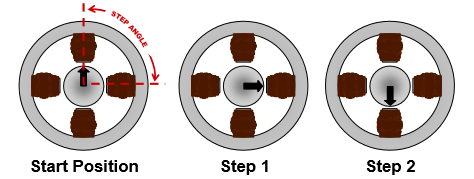
\includegraphics[width=\textwidth]{figures/move/motor1.png}
	\caption{Step Angle}
	\label{fig:angle} 
\end{figure}

Figure \ref{fig:angle} represents a stepper motor that requires 4 steps to complete a 360$^\circ$ 
rotation. This determines the step angle to be 90$^\circ$.
\newpage
The main components of a stepper motor are represented in Figure \ref{fig:main_components}, and 
they consist of stators, windings(phases), and rotor.
Attached to the output axle is the rotor, depending on the type of motor it can be magnetized.

\begin{figure}[htp]
	\centering
	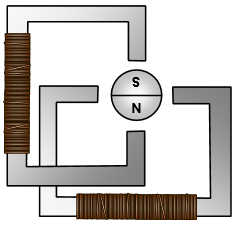
\includegraphics[width=0.3\textwidth]{figures/move/motor2.png}
	\caption{Main Components}
	\label{fig:main_components}
\end{figure}


By applying a voltage across one of the windings, current will start flowing through it. Using 
the right-hand rule, the direction of the magnetic flux can be determined. The flux will want to 
travel through the path that has the least resistance. This determines the rotor to change its 
position to minimize resistance. This is shown in Figure \ref{fig:flux}.

\begin{figure}[htp]
	\centering
	\subfloat[High Resistance]{%
		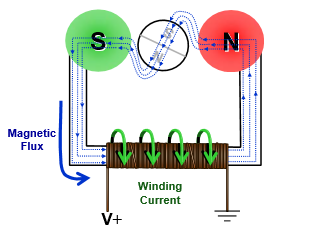
\includegraphics[width=0.4\textwidth]{figures/move/motor3.png}%
		}%
	\hfill
	\subfloat[Low Resistance]{%
		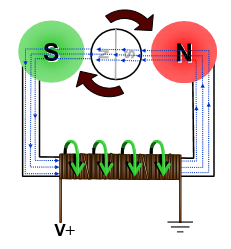
\includegraphics[width=0.4\textwidth]{figures/move/motor4.png}
	}
	\caption{Direction of Magnetic Flux}
	\label{fig:flux}
\end{figure}
\newpage
\subsection{Types of Stepper Motors}
\subsubsection{Permanent Magnet Motor}
This type of stepper motor has a magnetized rotor. Each winding will be subdivided into two, to 
better understand how to motor functions. Figure \ref{fig:bas_struct} represents the windings, and 
how they are distributed inside a stepper motor.

\begin{figure}[htp]
    \centering
    \subfloat[Rotor]{%
        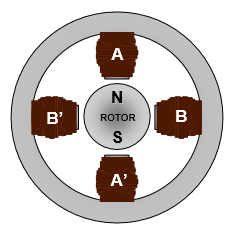
\includegraphics[width=0.4\textwidth]{figures/move/motor5.png}%
        }%
    \hfill%
    \subfloat[Winding]{%
        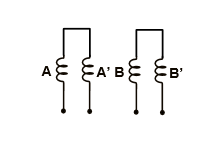
\includegraphics[width=0.4\textwidth]{figures/move/motor6.png}%
        }%
    \caption{Basic Structure of a Motor}
    \label{fig:bas_struct} 
\end{figure}

The resolution of the motor can be improved in two ways, either by increasing the number of pole 
pairs in the rotor itself, or by increasing the number of phases as shown in Figure 
\ref{fig:inc_res}.


\begin{figure}[htp]
    \centering
    \subfloat[Increased Pole Pairs]{%
        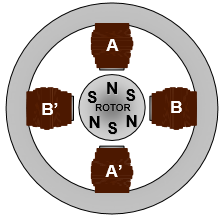
\includegraphics[width=0.4\textwidth]{figures/move/motor7.png}%
        }%
    \hfill%
    \subfloat[Increased Number of Winding]{%
        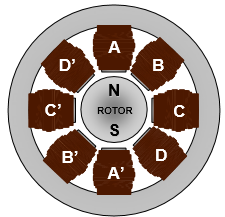
\includegraphics[width=0.4\textwidth]{figures/move/motor8.png}%
        }%
	\hfill%
	\caption{Increased resolution}
	\label{fig:inc_res}
\end{figure}

\newpage
To rotate the motor, simply apply a voltage across the windings in a sequence. A full rotation is 
shown in Figure \ref{fig:stepping_perm_magn}, with the corresponding phases energized.

\begin{figure}[htp]
    \begin{center}
    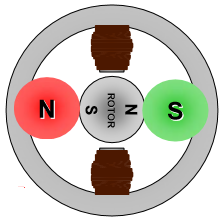
\includegraphics[width=0.2\textwidth]{figures/move/motor9.png}    
    \hfill
    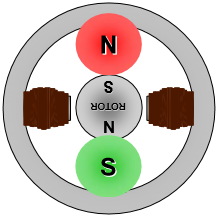
\includegraphics[width=0.2\textwidth]{figures/move/motor10.png}
    \hfill
    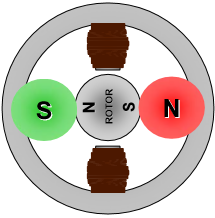
\includegraphics[width=0.2\textwidth]{figures/move/motor11.png}
  	\hfill
  	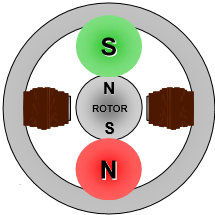
\includegraphics[width=0.2\textwidth]{figures/move/motor12.png}
    \end{center}
\end{figure}
\vspace{-10mm}
\begin{figure}[htp]
    \begin{center}
    \subfloat[$1\textsuperscript{st}$ Step]{
        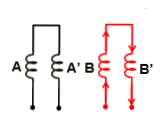
\includegraphics[width=0.2\textwidth]{figures/move/motor13.png}
        }
    \hfill
    \subfloat[$2\textsuperscript{nd}$ Step]{
        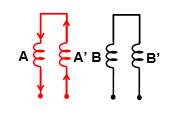
\includegraphics[width=0.2\textwidth]{figures/move/motor14.png}
        }
    \hfill
    \subfloat[$3\textsuperscript{rd}$ Step]{
    	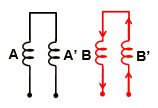
\includegraphics[width=0.2\textwidth]{figures/move/motor15.png}
    	}
  	\hfill
  	\subfloat[$4\textsuperscript{th}$ Step]{
  		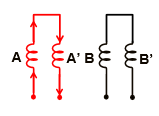
\includegraphics[width=0.2\textwidth]{figures/move/motor16.png}
  		}
  	\caption{Stepping a Permanent Magnet Motor}
  	\label{fig:stepping_perm_magn}
    \end{center}
\end{figure}
\subsubsection{Variable Reluctance Motor}
This type of motor uses a rotor that is not magnetized, and has a number of teeth as seen in 
Figure \ref{fig:var_rel_components}. The windings are configured differently, as depicted in 
\ref{fig:var_rel_components}(b), all having a common voltage source but separate ground 
connections.
They usually have 3 or 5 windings.
Greater precision can be achieved by adding more teeth to the rotor.

\begin{figure}[htp]
    \centering%
    \subfloat[Non Magnetized Rotor]{%
        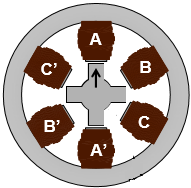
\includegraphics[width=0.3\textwidth]{figures/move/motor17.png}%
        }%
    \hfill%
    \subfloat[Windings]{%
        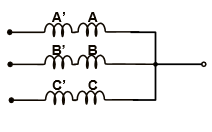
\includegraphics[width=0.4\textwidth]{figures/move/motor18.png}%
        }%
    \caption{Variable Reluctance Motor Components}%
    \label{fig:var_rel_components}%
\end{figure}
\newpage

To spin the motor, each winding is energized one at a time, and the rotor rotates to minimize 
reluctance as explained before.
Some of the differences, between this type of stepper motor and the permanent magnet motor, are 
that, in order to spin the motor in a direction, the windings have to be energized in a reverse 
sequence as opposed to the direction of the spin, as depicted in Figure \ref{fig:stepping_var_rel}.

In addition, variable reluctance motors have twice the precision of permanent magnet motors with 
the same amount of windings.
\begin{figure}[htp]
    \begin{center}
    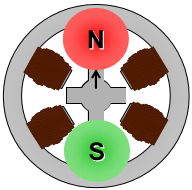
\includegraphics[width=0.2\textwidth]{figures/move/motor19.png}
    \hfill
    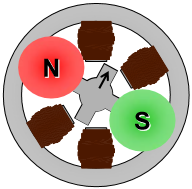
\includegraphics[width=0.2\textwidth]{figures/move/motor20.png}
    \hfill
    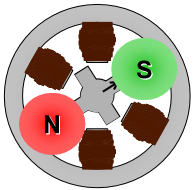
\includegraphics[width=0.2\textwidth]{figures/move/motor21.png}
  	\hfill
  	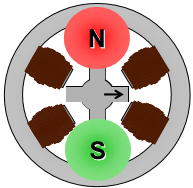
\includegraphics[width=0.2\textwidth]{figures/move/motor22.png}
	\end{center}
	\begin{center}
    \subfloat[$1\textsuperscript{st}$ Step]{
        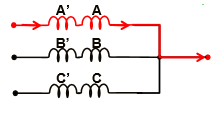
\includegraphics[width=0.2\textwidth]{figures/move/motor23.png}
        }
    \hfill
    \subfloat[$2\textsuperscript{nd}$ Step]{
        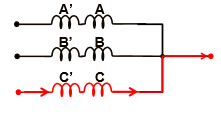
\includegraphics[width=0.2\textwidth]{figures/move/motor24.png}
        }
    \hfill
    \subfloat[$3\textsuperscript{rd}$ Step]{
    	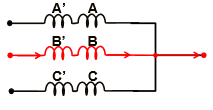
\includegraphics[width=0.2\textwidth]{figures/move/motor25.png}
    	}
  	\hfill
  	\subfloat[$4\textsuperscript{th}$ Step]{
  		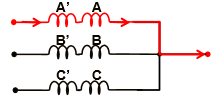
\includegraphics[width=0.2\textwidth]{figures/move/motor26.png}
  		}
  	\caption{Stepping Variable Reluctance Motor}
  	\label{fig:stepping_var_rel}
  	\end{center}
\end{figure}
\newpage
\subsubsection{Hybrid Stepper Motor}
Hybrid stepper motors borrow characteristics from both previously mentioned types.

Figure \ref{fig:hybrid_components} shows the two the main components of the hybrid stepper motor. 
On the left side, the stator can be seen consisting of 8 poles. On the right side the rotor. The 
rotor consists of two sets of teeth, corresponding to the two poles, north and south.
\begin{figure}[h]
	\centering
	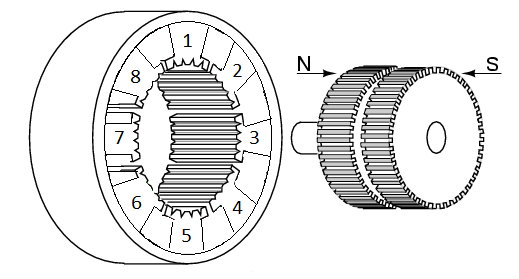
\includegraphics[width=\textwidth]{figures/move/motor27.png}
	\caption{Stator and Rotor}
	\label{fig:hybrid_components}
\end{figure}

It is important to notice two additional things. The first, is that the teeth on the rotor are not 
aligned but are interleaved. The second, is the placement of the stator teeth in respect to those 
of the rotor. Both can be observed in Figure \ref{fig:stepper}.

\begin{figure}[htp]
    \centering%
    \subfloat[Interleaved Teeth]{%
        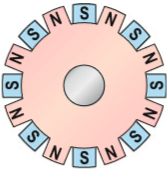
\includegraphics[width=0.4\textwidth]{figures/move/motor28.png}%
        }%
    \hfill%
    \subfloat[Stepper Motor Inside]{%
        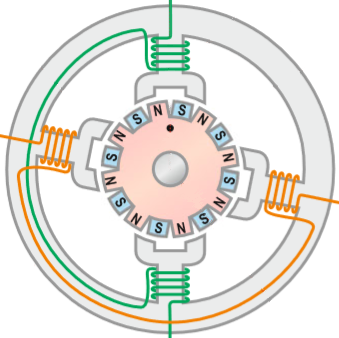
\includegraphics[width=0.3\textwidth]{figures/move/motor29.png}%
        }%
    \caption{Hybrid Stepper Motor}
    \label{fig:stepper}
\end{figure}
\newpage
Figure \ref{fig:stepper}, the windings with numbers 1 and 5 are completely aligned with the teeth 
of the rotor. Windings number 3 and 7 are completely unaligned, while the others are half aligned. 
This results in higher precision and higher torque offered by the hybrid stepper motor, depending 
on the stepping method used.

Figures \ref{fig:hybrid_first_step},  \ref{fig:hybrid_second_step}, \ref{fig:hybrid_third_step},
\ref{fig:hybrid_forth_step} 
represent the way this motor operates.

\begin{center}
	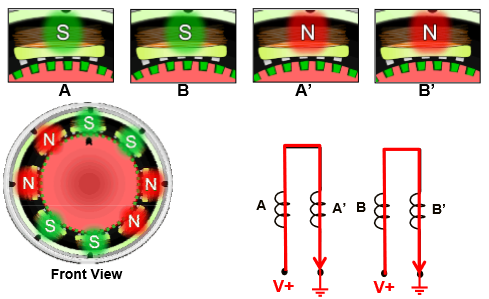
\includegraphics[width=0.8\textwidth]{figures/move/motor32}
	\captionof{figure}{First Step}
	\label{fig:hybrid_first_step}
\end{center}
By applying a voltage to both windings, the current flow can be controlled, thereby controlling the 
polarity of each stator pole, thus controlling the direction of the motor. Notice that, initially, 
poles A and A’ are completely aligned, and poles B and B’ are half aligned. 

\begin{center}
	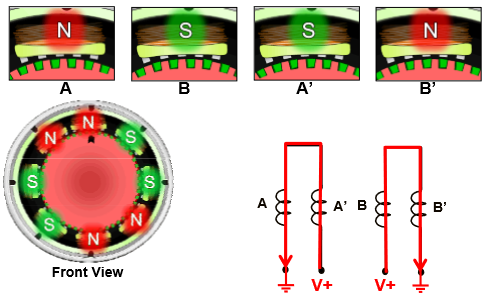
\includegraphics[width=0.8\textwidth]{figures/move/motor33}
	\captionof{figure}{Second Step}
	\label{fig:hybrid_second_step}
\end{center}

Next step involves changing the direction of the current in winding A by applying a voltage at the 
other end of the winding. Even though only the current in winding A has been changed, all stator 
poles are aligned differently. Poles A and A’ are now half aligned, and poles B and B’ are 
completely aligned.

\begin{center}
	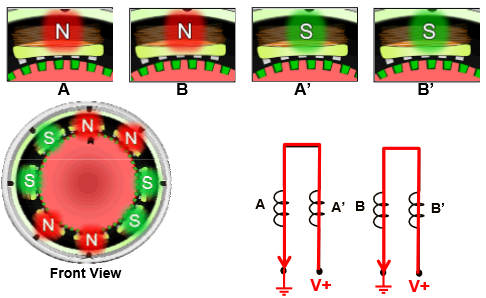
\includegraphics[width=0.8\textwidth]{figures/move/motor34}
	\captionof{figure}{Third Step}
	\label{fig:hybrid_third_step}
\end{center}

Now, changing the direction of the current in winding B, changes the polarity of the stator poles B 
and B', again, determining a change in the alignment of all stator poles. A and A’ are now 
completely aligned, and stator poles B and B’ are half aligned. The positions of the stator poles 
now correspond to those of the first step.

\begin{center}
	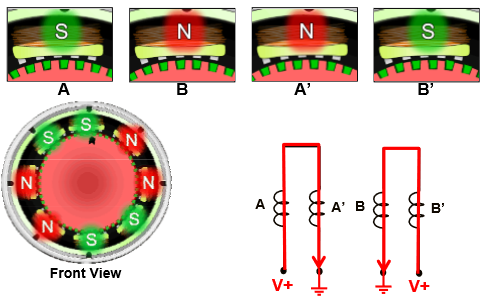
\includegraphics[width=0.8\textwidth]{figures/move/motor35}
	\captionof{figure}{Forth Step}
	\label{fig:hybrid_forth_step}
\end{center}


Finally, again changing the direction of the current in winding A, determines the rotor to move 
another step. Notice the alignment of the stator poles. A and A’ are half aligned, while B and B’ 
are fully aligned. By changing the direction of the current in winding B, the motor arrives in the 
initial state, thus repeating the sequence.


\subsection{Unipolar And Bipolar Stepper Motors}

Another classification of stepper motors, is depending on the way the windings are configured.
Even though, nowadays, almost every stepper is both.
Meaning that unipolar and bipolar, are rather modes in which the stepper motor can be driven.
Exception being, stepper motors which have only four wires coming out of them, corresponding to 
bipolar stepper motors.

Figure \ref{fig:windings} below represent the configuration of the windings in both unipolar and 
bipolar stepper motors. 


\begin{figure}[htp] 
    \centering
    \subfloat[Bipolar]{
        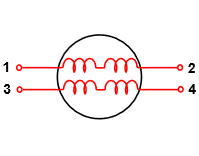
\includegraphics[width=0.4\textwidth]{figures/move/motor37.png}
        }
    \hfill
    \subfloat[Unipolar]{%
        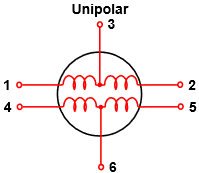
\includegraphics[width=0.4\textwidth]{figures/move/motor36.png}
        }
    \caption{Winding Configuration}
    \label{fig:windings}
\end{figure}

Bipolar stepper motors have one winding per phase. To energize the first phase, voltage needs to 
be applied to lead 1, and lead 2 needs to be connected to ground. Stepping the motor, 
involves energizing one phase, then the second, then the first phase again with reverse
polarity, meaning the voltage source and the ground must be switched between each other(lead 1 – 
ground, lead 2 – voltage source). Afterwards, the second winding is energized with reverse 
polarity. This makes driving them more difficult. We use driver boards to make the task easier. 

Unipolar stepper motors allow current flow in only one direction through the winding, unlike 
bipolar stepper motors. Because of that, a center wire has been added to each winding corresponding 
to leads 3 and 6. All the other leads are connected to ground. Outside the motor, each lead 
connected to ground is connected to a transistor first. To step the motor, apply voltage to 
the corresponding transistor to connect the lead to ground and allow current flow 
through that winding.  
\newpage
Note that the bipolar configuration as shown in Figure \ref{fig:bipolar_stepping} allows the 
current to flow in both directions, but the voltage and ground continuously switch positions. This 
makes bipolar stepper motors a bit more complicated to drive, but as previously stated, motor 
driver boards simplify the task.

\begin{figure}[htp] 
    \centering
    \subfloat[$1\textsuperscript{st}$ Step]{
        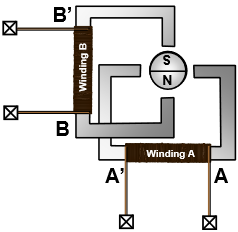
\includegraphics[width=0.3\textwidth]{figures/move/motor43.png}
        }
    \hfill
    \subfloat[$2\textsuperscript{nd}$ Step]{
        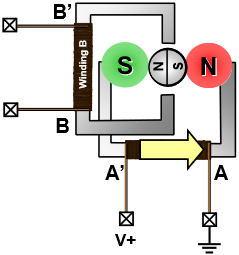
\includegraphics[width=0.3\textwidth]{figures/move/motor44.png}
        }
    \hfill
    \subfloat[$3\textsuperscript{rd}$ Step]{
    	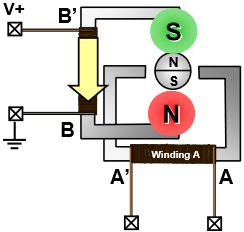
\includegraphics[width=0.3\textwidth]{figures/move/motor45.png}
    	}
   	\hfill
   	\subfloat[$4\textsuperscript{th}$ Step]{
  		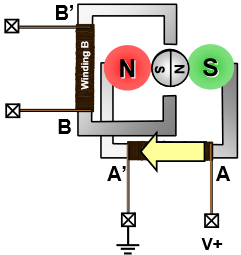
\includegraphics[width=0.3\textwidth]{figures/move/motor46.png}
  		}
  	\hfill
  	\subfloat[$5\textsuperscript{th}$ Step]{
  		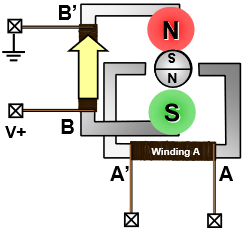
\includegraphics[width=0.3\textwidth]{figures/move/motor47.png}
  		}
  	\caption{Bipolar Motor Spinning}
  	\label{fig:bipolar_stepping}
\end{figure}
%\section{Tri-State Buffer}\label{sec:buffer}
\subsection{Motor Driver Boards}\label{sec:driver_boards}
We used motor driver boards in order to drive the motors. They provide a simple interface between 
the microcontroller and the motors, and make for a better alternative than directly driving the 
motors from the microcontroller.
\begin{figure}[htp]
	\centering
	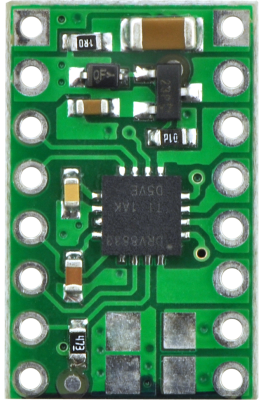
\includegraphics[scale=0.6]{figures/move/driver_board}
	\caption{Driver Board}
\end{figure}
\section{Wheels}\label{sec:wheels}
The robot should be able to move in eight directions from every position.
By using traditional wheels, the robot would need to be able to steer to the desired direction, 
thus changing orientation.
This would have been a difficult task raising a number of problems.
Our solution is to use omni-wheels instead.
A standard wheel and an omni-wheel are shown in Figure \ref{fig:wheels}.

The key difference between omni-wheels and traditional wheels is their contact area.
For omni-wheels it consists of smaller wheels that are able to move freely sideways,
thus not generating any friction.

\begin{figure}[htp]
	\centering
	\subfloat[Standard Wheel]{
		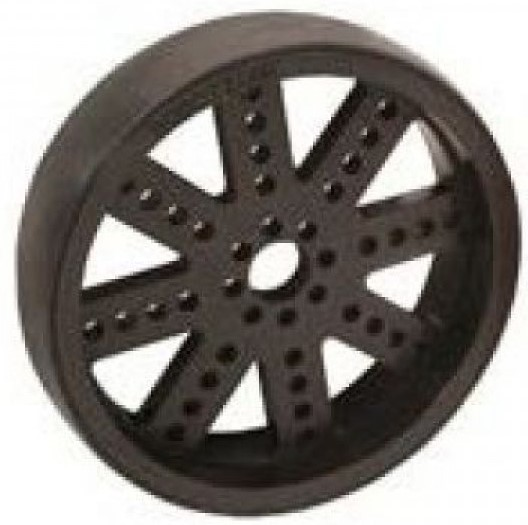
\includegraphics[width=0.2\textwidth]{figures/move/regular_wheel}
	}
	\hspace{0.2\textwidth}
	\subfloat[Omni-Wheel]{
		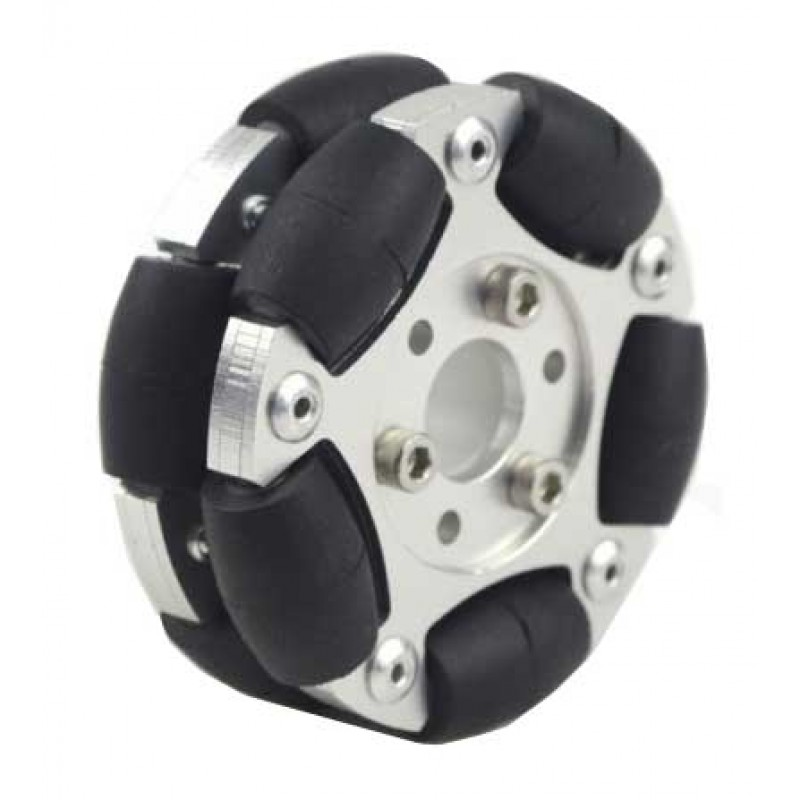
\includegraphics[width=0.2\textwidth]{figures/move/omni_wheel}
	}
	\caption{Wheels}
	\label{fig:wheels}
\end{figure}
By mounting the wheels in pairs, with the shafts crossing at a 90$^\circ$ angle, we are able to 
move the robot in any direction without needing to change the orientation of the robot.
This is achieved through rotating the pairs as shown in figure \ref{fig:forces}.
\begin{figure}[htp]
	\begin{center}
    \subfloat[North]{
    	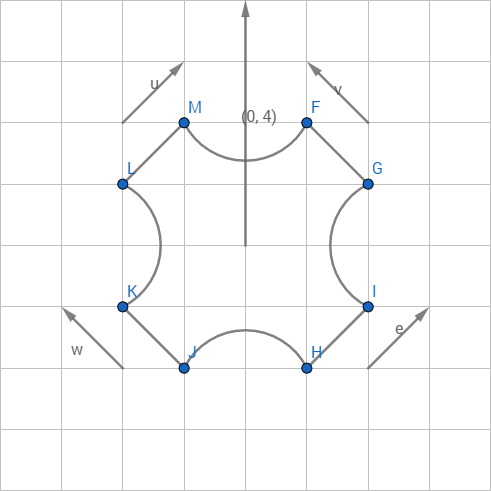
\includegraphics[width=0.2\textwidth]{figures/move/vector_addition_North}
    }
    \subfloat[East]{
    	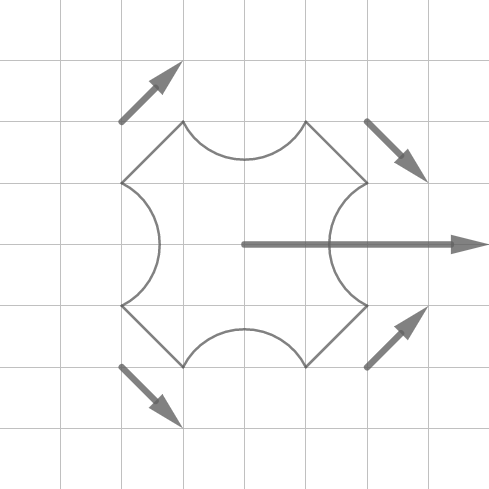
\includegraphics[width=0.2\textwidth]{figures/move/vector_addition_East}
    }
    \subfloat[South]{
   		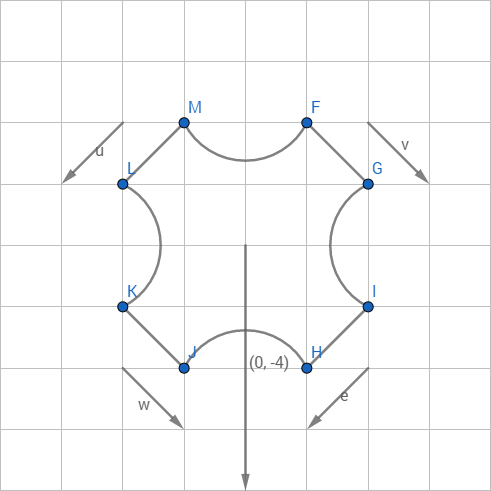
\includegraphics[width=0.2\textwidth]{figures/move/vector_addition_South}
    }
  	\subfloat[West]{
 		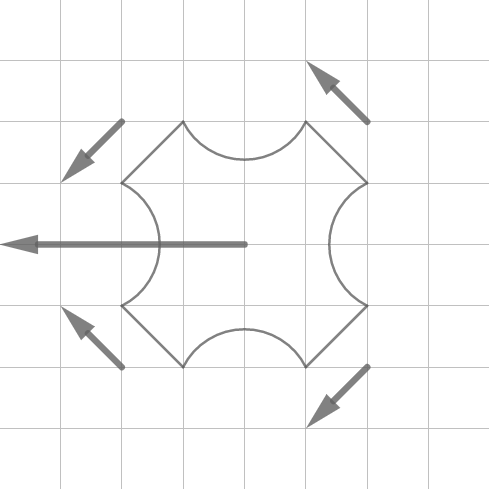
\includegraphics[width=0.2\textwidth]{figures/move/vector_addition_West}
	}
	\end{center}
	\vspace{-5mm}
	\begin{center}
    \subfloat[North-East]{
    	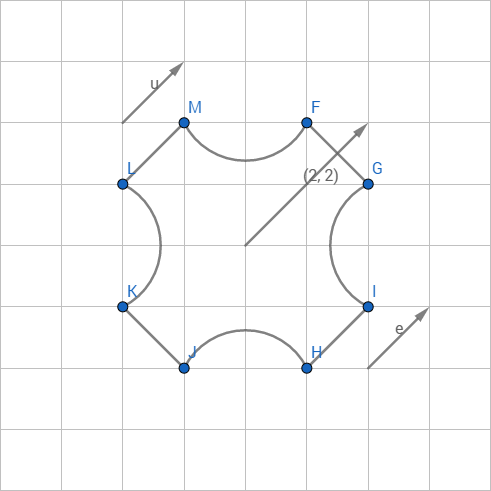
\includegraphics[width=0.2\textwidth]{figures/move/wheel_vectors_NE}
    }
    \subfloat[South-East]{
   		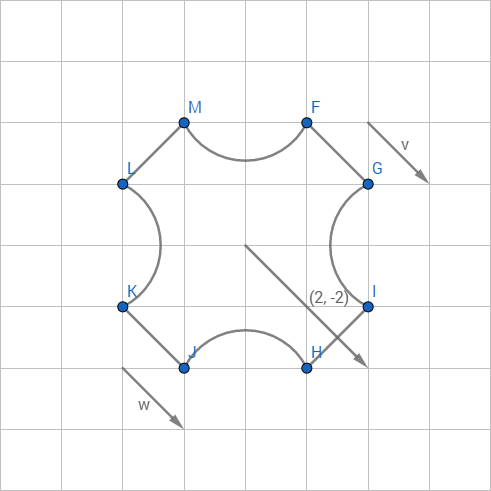
\includegraphics[width=0.2\textwidth]{figures/move/wheel_vectors_SE}
    }
    \subfloat[South-West]{
    	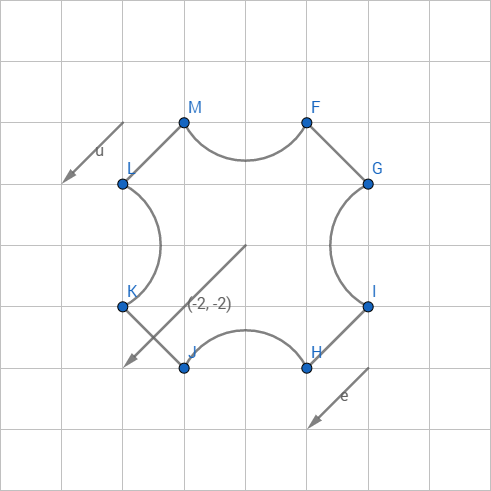
\includegraphics[width=0.2\textwidth]{figures/move/wheel_vectors_SW}
    }
  	\subfloat[North-West]{
  		\includegraphics[width=0.2\textwidth]{figures/move/wheel_vectors_NW}
	}
	\end{center}
	\vspace{-5mm}
  	\caption{Forces from Multiple Wheels Added Together}
  	\label{fig:forces}
\end{figure}
\newpage
It can also be observed that no two opposite motors spin in different directions,
because this would lead to a rotation, which is undesired for us.
This has also made our task of programming the motors more simple.
\newpage
\section{Direction Control}\label{sec:direction}
To decide the direction of the robot, we had to control which wheels turn what number of steps. 

One option would have been to control each motor individually.
This required four pins for each motor to step the motors,
and precise timing between the four motors.
Imprecise timing could introduce unintended rotation.

We decided to build our own circuit using tri-state buffers instead.
The circuit will be explained after a short explanation of tri-state buffers.

%This would drastically lower the number of pins needed, and would make for a more precise and 
%advanced way of driving the motors.

\subsection{Tri-State Buffer}
To achieve the desired movement using as few pins as possible, we decided to use Tri-State buffers.
Fewer pins make it easier to port this part of the robot to a smaller $\mu$C with fewer pins for a 
final product.

Tri-State buffers provide the possibility of disconnecting parts of the circuit, when not needed.
This allowed us to manipulate the input to the motors dynamically.

A Tri-State buffer can be thought of as a switch. Figure \ref{fig:tristate} better illustrates that 
concept.
\begin{figure}[htp]
	\begin{center}
	\subfloat[Disabled]{
		\includegraphics[width=0.3\textwidth]{figures/move/motor48}
		}
	\hspace{2cm}
	\subfloat[Enabled]{
		\includegraphics[width=0.3\textwidth]{figures/move/motor49}
		}
	\caption{Tri-State Buffer Switch Analogy}
	\label{fig:tristate}
	\end{center}
\end{figure}


When the buffer is enabled, its output corresponds to its input, either 0 or 1, "High" or "Low".
However when the buffer is a in its third state, its output is disabled, opening the circuit 
between the buffer and the next component.
That does not mean its output corresponds to a logic “Low", but instead it is in a state of high 
impedance in which the output is disconnected from the rest of the circuit.
\newpage
\subsection{Control Circuit}\label{sub:circuit}
Initially, we have thought of a movement system,
which required 16 pins to accommodate moving in all directions.
In this system we would have controlled each motor individually,
requiring 4 pins for each motor.
With this method,
it would have been necessary to have precise timing between the four stepping sequences.

Having a limited number of pins available, has forced us to think of the movement system very thoroughly.
The reason for this was that we wanted to test the movement system on the MSP430 $\mu$-C,
which only has 9 usable pins.
\todo{reference to msp}

Figure \ref{fig:mot_ctrl} shows a schematic of the motor control circuit.
\begin{figure}[htp]
	\centering
	\includegraphics[width=0.8\textwidth]{figures/move/direction_choice}
	\caption{Motor Control Circuit}
	\label{fig:mot_ctrl}
\end{figure}

The four wires coming from the microcontroller,
labeled '1', '2', '3' and '4' correspond to the stepping sequence.
They are connected to two Tri-State buffers corresponding to each pair of motors.
The location of the motors is shown in Figure \ref{fig:motor_pairs_location}.

\begin{figure}[htp]
	\centering
	\includegraphics[width=0.2\textwidth]{figures/move/Motor_pairs_location.jpg}
	\caption{Motor Pairs}
	\label{fig:motor_pairs_location}
\end{figure}

\clearpage
The first two Tri-State buffers switch the pair on or off,
dependent on it being necessary for moving in a specific direction.
The input pins, labeled ‘A Enable’ and ‘B Enable’ go to the 
two Tri-State buffers connected to each motor pair. 

Afterwards, each enabling buffer is connected to two buffers that decide the direction,
one active-high and one active-low.
Those two buffers can be controlled by one bit,
because of their opposite enable voltage.

For example, when moving North-East, only ‘Pair A’ is needed.
‘A Enable’ will have a ‘High’ signal while ‘B Enable’ will have a ‘Low’ signal.
Next, applying a ‘Low’ signal to ‘A Direction’, 
reverses the wiring of the motors determining the robot move North-East.

Note that, when moving in a specific direction,
the motors that form a pair,
have to spin in opposite directions.
One spins clockwise, while the other spins counter-clockwise.
This was achieved by wiring one motor in reverse as shown in Figure \ref{fig:reverse_wiring}.
\begin{figure}[htp]
	\centering
	\includegraphics[width=0.8\textwidth]{figures/move/motor_pairs_cedar.png}
	\caption{Motor Wiring}
	\label{fig:reverse_wiring}
\end{figure}

It is important to specify, that the robot moves in said directions using the same 
programming only by maintaining the same
orientation as in Figure \ref{fig:motor_pairs_location}.

Tables \ref{tab:directions} and \ref{tab:directions_signal} show the configurations 
required for moving in any of the eight directions.
\begin{table}[htp]
	\centering
	\caption{Directions}
	\begin{tabular}{|l|l|l|}
		\hline
		Direction 	& Pair A 	& Pair B	\\
		\hline
		North 		& forward 	& forward \\
		East 		& forward 	& backward \\
		South 		& backward 	& backward \\
		West 		& backward 	& forward \\
		\hline
		North-East 	& forward 	& off \\
		South-East 	& off 		& backward \\
		South-West 	& backward 	& off\\
		North-West 	& off 		& forward \\
		\hline
	\end{tabular}
	\label{tab:directions}
\end{table}
\begin{table}[htp]
	\centering
	\caption{Direction Signals}
	\begin{tabular}{|l|c|c|c|c|}
		\hline
		Direction & $A_{Enable}$ & $A_{Direction}$ & $B_{Enable}$ & $B_{Direction}$ \\
		\hline
		North 		& 1 & 0 & 1 & 0 \\
		East 		& 1 & 0 & 1 & 1 \\
		South 		& 1 & 1 & 1 & 1 \\
		West 		& 1 & 1 & 1 & 0 \\
		\hline	
		North-East 	& 1 & 0 & 0 & x \\
		South-East 	& 0 & x & 1 & 0 \\
		South-West 	& 1 & 1 & 0 & x \\
		North-West 	& 0 & x & 1 & 1 \\
		\hline
	\end{tabular}
	\label{tab:directions_signal}
\end{table}
\vfill